\documentclass[pdf,PItalk,slideColor,colorBG,accumulate]{prosper}
%\usepackage[dvips]{color}
\usepackage{latexsym,pstricks,pst-node,pst-coil,epsf}
\usepackage{amsmath,amsfonts,amsbsy,amssymb}

%geoffs
%blends
%bruce
%autumn
%contemporain
%lignesbleues
%gyom

% Definition of new colors
\newrgbcolor{LemonChiffon}{1. 0.98 0.8}
\newrgbcolor{LightBlue}{0.68 0.85 0.9}

%\def\fntb{\fontfamily{ppl}\fontshape{it}\fontsize{8pt}{10pt}\selectfont}
%\def\fnt{\usefont{T1}{pcr}{b}{n}\fontsize{8pt}{10pt}\selectfont}

%\def\fnt{\fontfamily{ppl}\selectfont}

%\def\aaa{\fontfamily{ppl}\fontsize{12pt}{6pt}\selectfont}

%\def\fnt{\fontfamily{ppl}\fontsize{8pt}{6pt}\selectfont}

\newcommand{\slashed}[1]{\hbox{{$#1$}\llap{$/$}}}
\newcommand{\myit}{\usefont{T1}{ppl}{m}{it}\fontsize{8pt}{6pt}\selectfont}
\newcommand{\p}{\partial}
\newcommand{\wt}{\widetilde}
\newcommand{\ov}{\overline}
\newcommand{\md}{\mathcal{D}}

\slideCaption{Lorentz Violating SQED}

\title{\normalsize Lorentz Violating Supersymmetric Quantum Electrodynamics}
\institution{
%\it Perimeter Institute for Theoretical Physics
%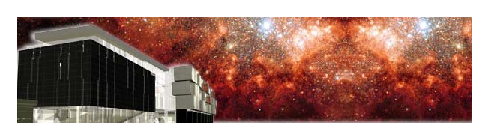
\includegraphics[width=10cm]{pi.eps}
%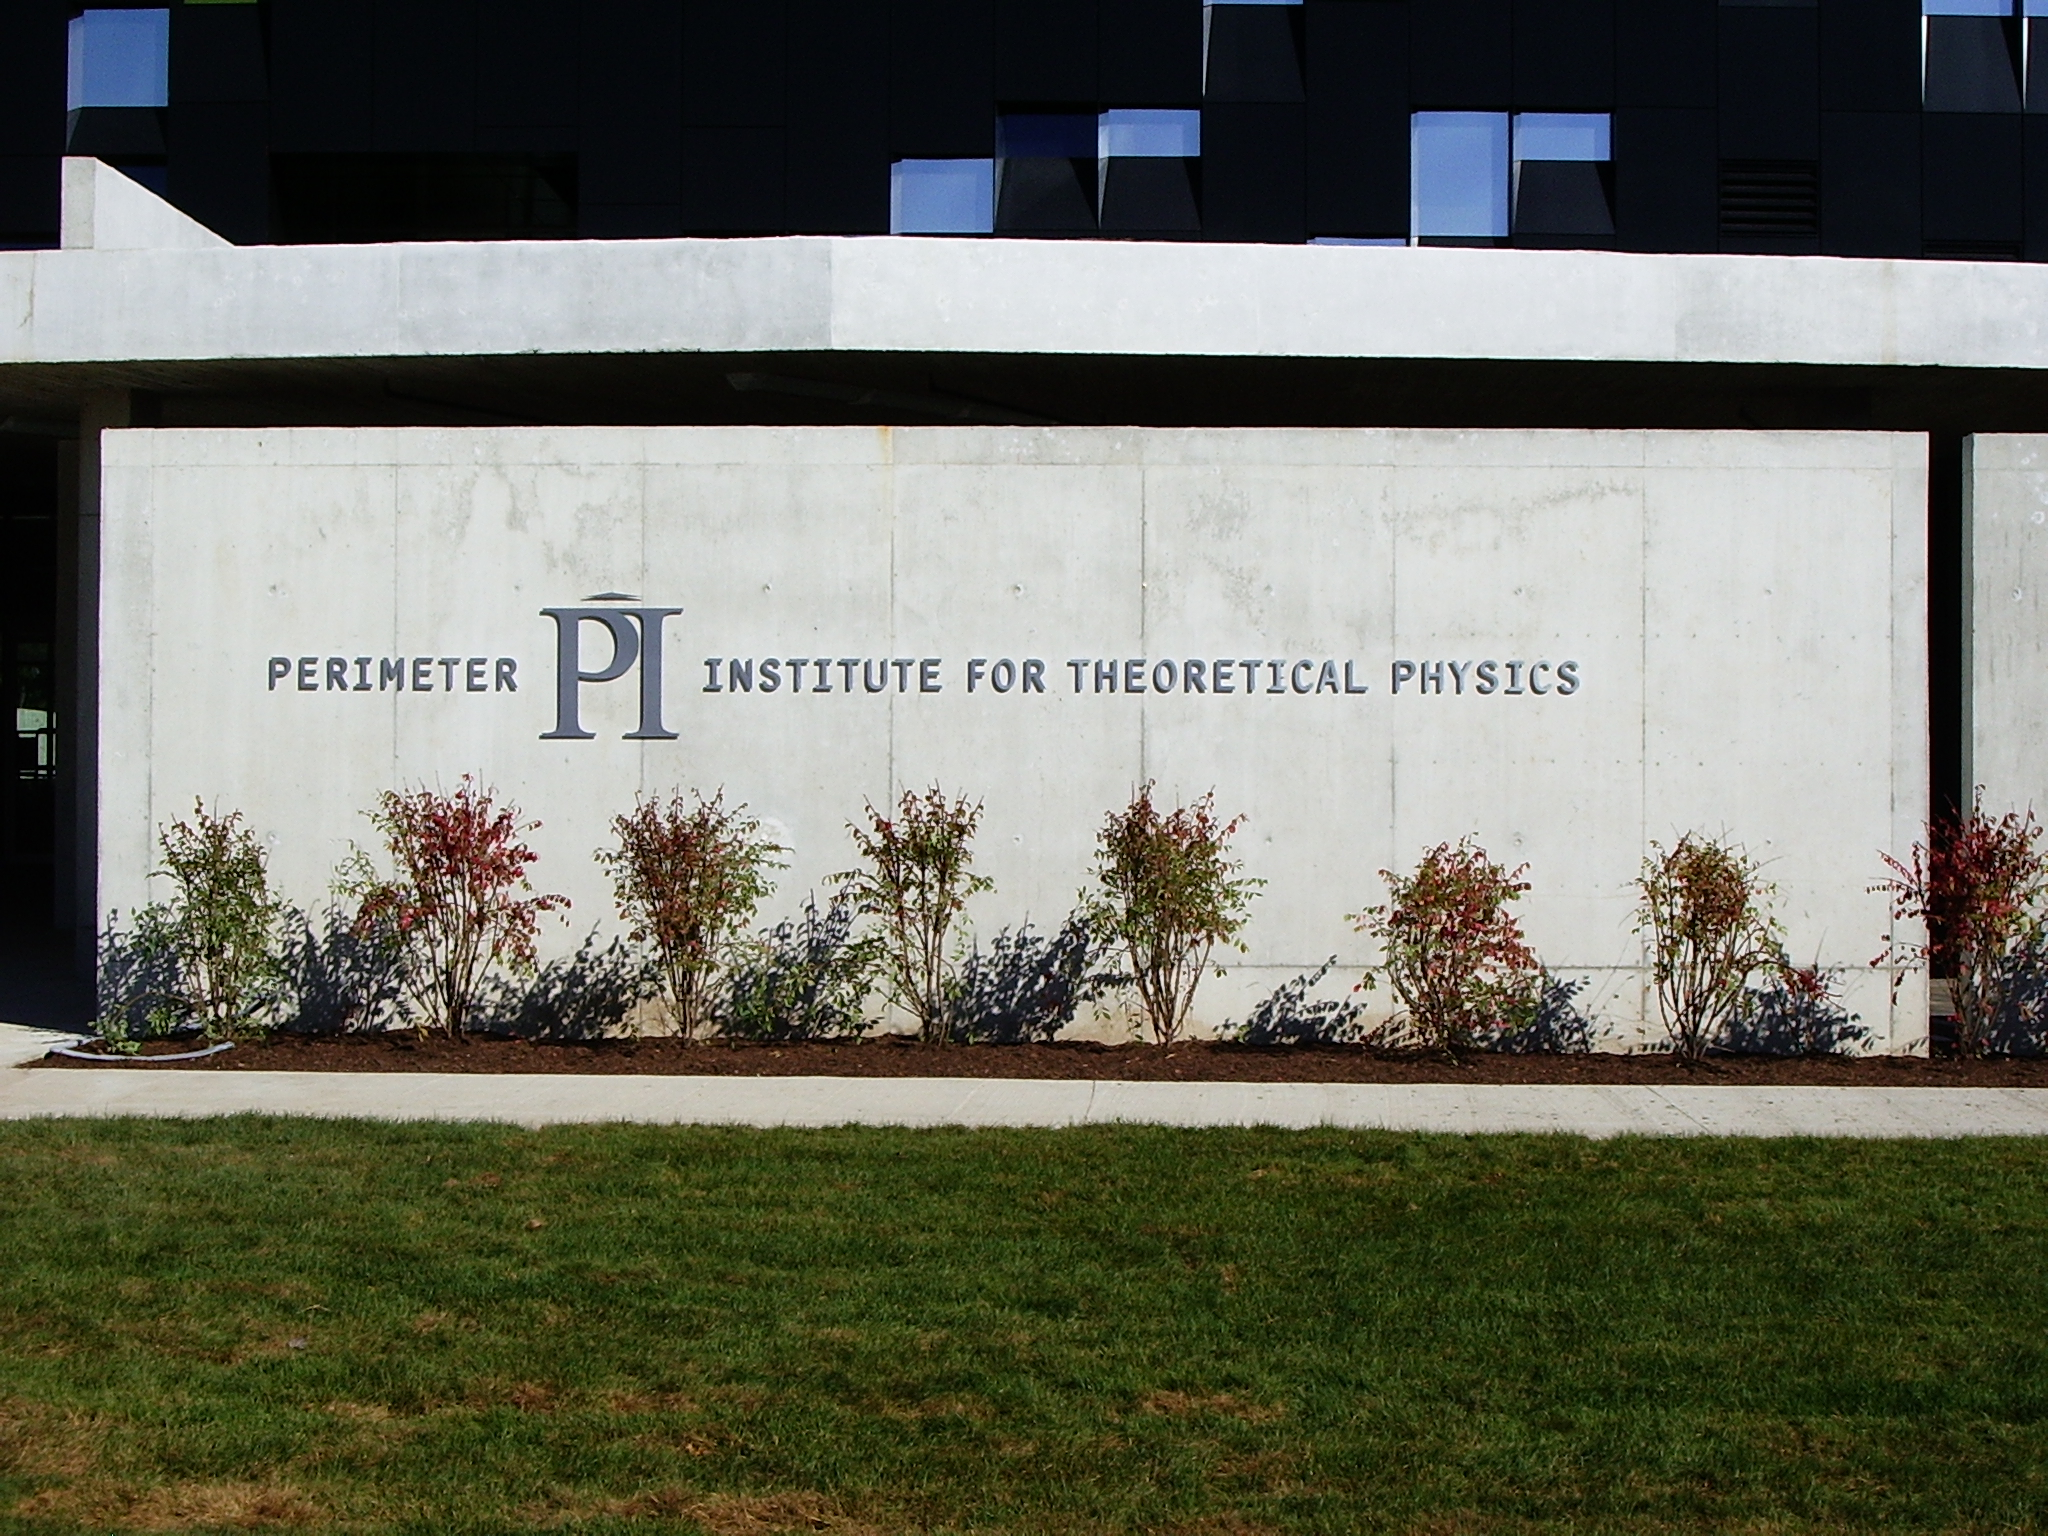
\includegraphics[width=10cm]{IMGP1870.EPS}
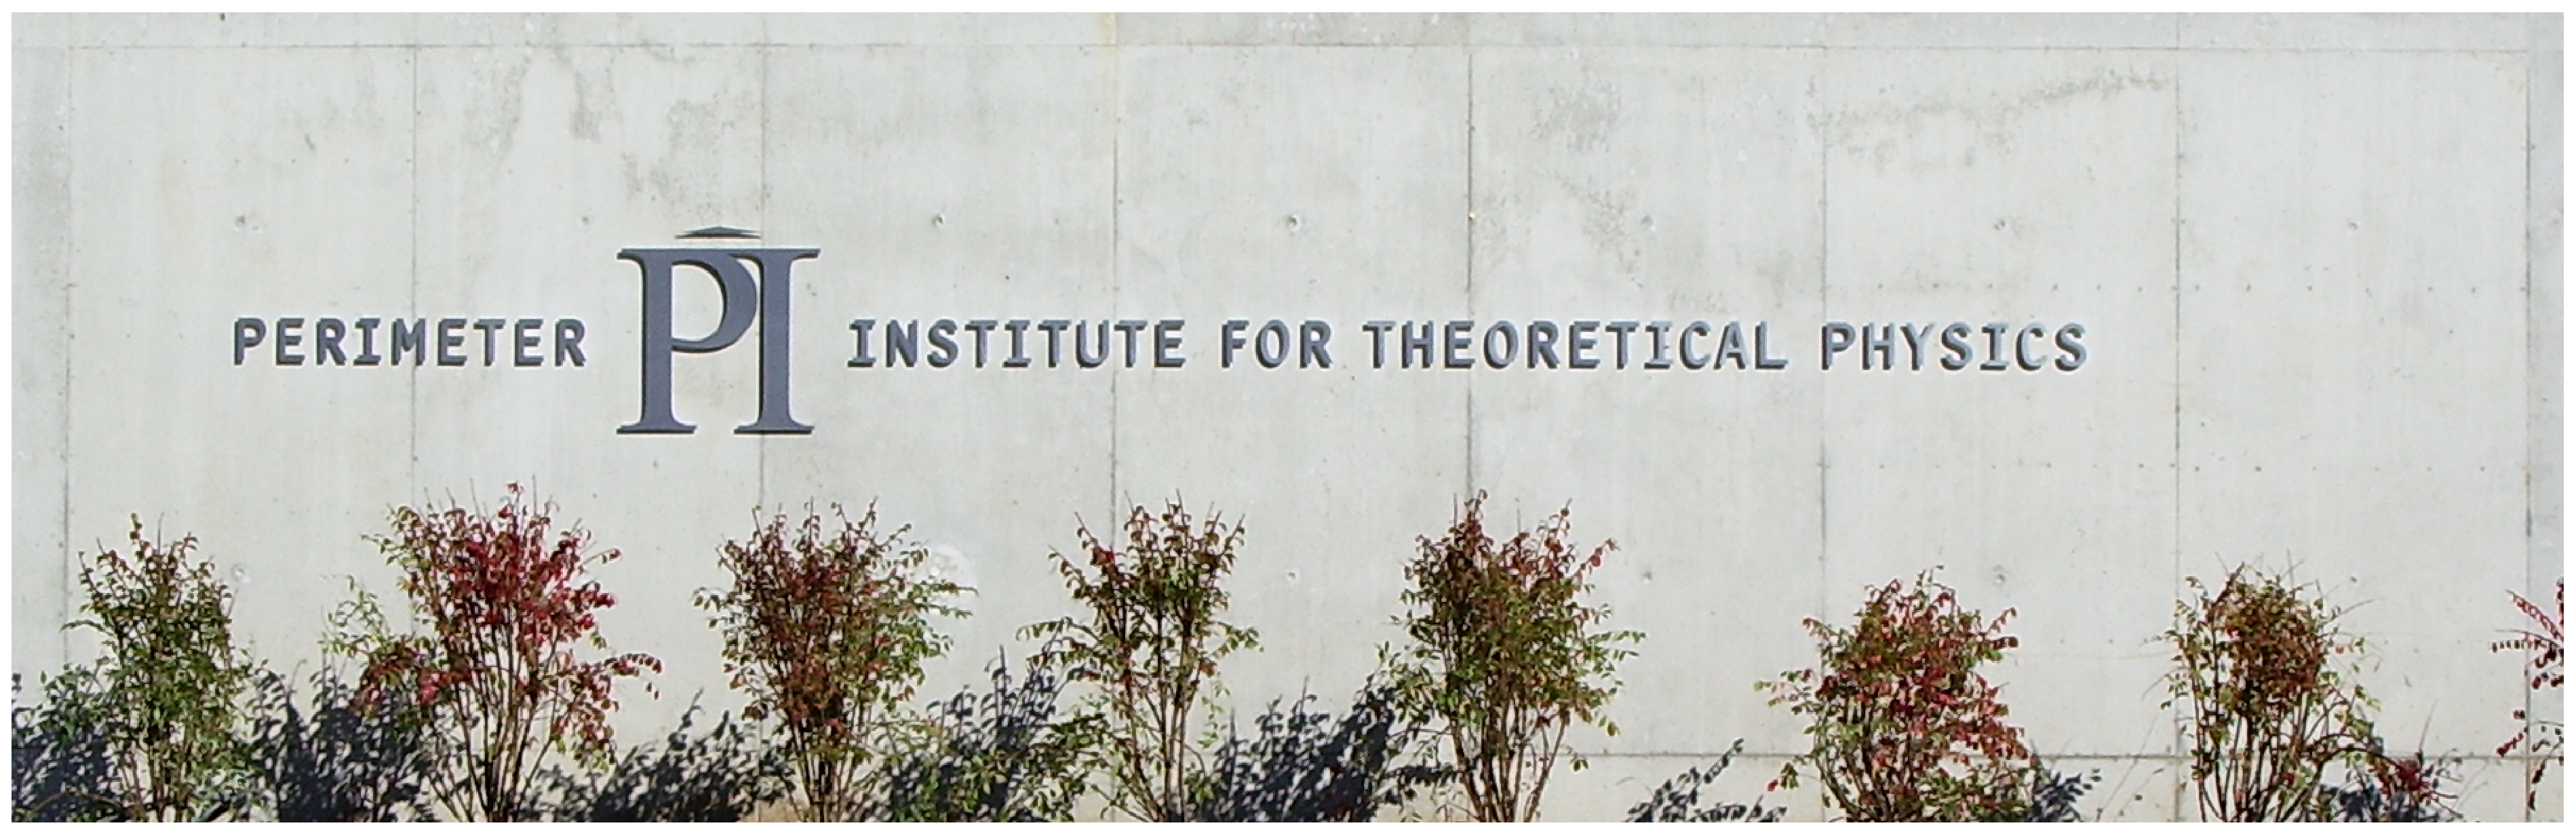
\includegraphics[width=9cm]{script.eps}
}
\author{Pavel A. Bolokhov}
 
\begin{document}
\maketitle

%%%%%%%%%%%%%%%%%%%%%%%%%%%%  SLIDE %%%%%%%%%%%%%%%%%%%%%%%%%%%%%%%%%%%%%%%

\overlays{5}
{
\begin{slide}{Introduction: Why Lorentz Violation?}
%\vspace{-0.5cm}
%\small
%\fnt
\onlySlide*{1}{
\DefaultTransition{Glitter}
}
\fromSlide*{2}
{
\DefaultTransition{Replace}
}

        There are many known examples in the history of physics when 
	a symmetry of nature, which was assumed to be exact, has fallen under
	experimental scrutiny.

	Lorentz symmetry is used as a crucial ingredient in the construction
	of fundamental theories of nature.

	There is a number of seemingly unrelated motives to study Lorentz
	violating theories:
\begin{itemstep}
\item Time evolution of dark energy (quintessence) 
      creates a preferred frame which could be detected as a LV 
 	background, provided that it couples to the Standard Model.
\item Low-energy limits of string theory contain
      a number of gauge fields with
        condensed fieldstrengths (fluxes) which
%(nearly) massless field, some of which
      carry open Lorentz indices.
\item There are some conjectures that a theory of Quantum Gravity
 	can manifest itself at low energies through LV modifications
	of particle dispersion relations.
\end{itemstep}

\fromSlide{4} 
{
	Direct experimental constraints on modifications of dispersion
	relations come from {\myit astrophysical processes} 
	\fromSlide{5}{and terrestrial 
	{\myit clock comparison} and 
	{\myit torsion balance} experiments.
	}
}

%\FromSlide{5}
%\begin{itemstep}
%	\item \fromSlide{4} {astrophysical processes}
%	\item \fromSlide{5} {terrestrial clock comparison}
%		\fromSlide{6} {and torsion balance experiments}
%\end{itemstep}
%	astrophysical processes and terrestrial
%	clock comparison and torsion balance 
%	experiments.
\end{slide}
}

%%%%%%%%%%%%%%%%%%%%%%%%%%%%  SLIDE %%%%%%%%%%%%%%%%%%%%%%%%%%%%%%%%%%%%%%%

\overlays{6}
{
\begin{slide}{\small Lorentz Violating EFT}
%\small
%\fnt
\onlySlide*{1}{
\DefaultTransition{Box}
}
\fromSlide*{2}
{
\DefaultTransition{Replace}
}

	One of the most straightforward ways to study the effects of
	new physics is to parametrize all our ignorance into a small 
	number of new parameters.

\FromSlide{2}
	In QED, the generic expansion in terms of the gauge invariant 
	operators starts at dimension {\red three}:

\[
\nonumber
{\cal L}_{\rm QED}^{(3)} =
~-~{\dgreen a_\mu}\,  \bar \Psi \gamma_\mu \Psi
~-~ {\dgreen b_\mu}\,  \bar \Psi \gamma^\mu \gamma_5 \Psi 
~-~ \frac{1}{2}{\dgreen H_{\mu\nu}}\bar \Psi \sigma^{\mu\nu} \Psi
~-~ {\dgreen k_\mu}\,  
\epsilon^{\mu\nu\kappa\lambda} A_\nu \partial_\kappa A_\lambda~.
%\label{LVqed}
\]

\FromSlide{3}
	Dimension three operators create a problem:
	from dimensional counting one expects 
	{\blue $ a_\mu \sim M n_\mu $}, 
	where {\blue $ n_\mu $} is a unit vector, and
	$ M $ is the scale of New Physics.
	That creates {\myit\blue disastrous} effects.

\FromSlide{4}
	Even if the LV coefficients are tuned small, they will be 
	exploded by quantum corrections coming from quadratic divergencies
	of the higher-dimensional operators:
\FromSlide{5}
\[
[LV]_{\rm dim~3} ~~\sim~~ ({\rm loop~factor}) \, 
\;\Lambda_{UV}^2\;
\times\; [LV]_{{\rm dim}~5}~. 
\]

	Dimension five operators have to be tuned too \quad
	$ \Longrightarrow $ \quad no room for LV interactions.

\FromSlide{6}
	One of the solutions is if such quadratic divergencies
	are suppressed by a {\red symmetry}.

\end{slide}
}

%%%%%%%%%%%%%%%%%%%%%%%%%%%%  SLIDE %%%%%%%%%%%%%%%%%%%%%%%%%%%%%%%%%%%%%%%
\overlays{5}
{
\begin{slide}[Replace]{\small Supersymmetry \fromSlide{5}{rules!}}

	Recently it has been proposed that SUSY could provide a 
	powerful selection rule on admissible forms of LV interactions.

\FromSlide{2}
	In particular in the Minimal Supersymmetric Standard Model,
	LV operators of dimensions three and four are prohibited
	by the requirements of supersymmetry and gauge invariance.

	Lorentz-violating interactions start only at dimension five.

\FromSlide{3}
	Once Supersymmetry is softly broken, dimension three LV
	operators can be induced, with coefficients controlled
	by the soft-breaking mass scale, 
	{\red $ m_s \sim 1~{\rm TeV} $}.	

\FromSlide{4}
	Dimension three operators are now pure quantum effects, and
	effectively, the divergencies are stabilized at the 
	supersymmetric threshold:
\[
[LV]_{\rm dim~3} ~~\sim~~ ({\rm loop~factor}) \, 
\;{\red m_{s}^2}\;
\times\; [LV]_{{\rm dim}~5}~.
\]
\FromSlide{5}
	$ \Rrightarrow $ This might lead to a solution of the
	naturalness problem: why the lower dimensional LV operators
	are so much suppressed as compared to their natural scale.

%%\rnode{left1}{\strut}
%%\[
%%\nonumber
%%{\cal L}_{\rm QED}^{(3)} = 
%%~-~{\black a_\mu}\,  \bar \Psi \gamma_\mu \Psi
%%~-~ {\black b_\mu}\,  \bar \Psi \gamma^\mu \gamma_5 \Psi 
%%~-~ \frac{1}{2}{\black H_{\mu\nu}}\bar \Psi \sigma^{\mu\nu} \Psi
%%~-~ {\black k_\mu}\,  
%%\epsilon^{\mu\nu\kappa\lambda} A_\nu \partial_\kappa A_\lambda~.
%%\]
%%\rnode{right1}{\strut}
%%\ncline[linecolor=red]{left1}{right1}
\end{slide}
}
%%%%%%%%%%%%%%%%%%%%%%%%%%%%  SLIDE %%%%%%%%%%%%%%%%%%%%%%%%%%%%%%%%%%%%%%%
\overlays{10}
{
\begin{slide}[Replace]{\small Questions we ask}

\fromSlide{1}{
	In our work we have set up the following objectives, confining
	ourselves to SQED, but being on a path to the full 
	Lorentz-violating MSSM:
	}
\begin{itemstep}
	\item 
	\fromSlide{2}
	{prove the absence of the naturalness problem in the LV sector}
	\item 
	\fromSlide{3}{
	derive phenomenological constraints on the LV parameters
		of SQED}
\end{itemstep}

\fromSlide{4}{	
	In detail, the investigation includes:}
\begin{itemstep}
	\item 
	\fromSlide{5}{
		find out whether D-term anomaly (cancellation) is disturbed
		by the presence of LV interactions}
	\item 
	\fromSlide{6}{
	prove that gauge anomaly does not arise due to 
      	      the LV interactions}
	\item
	\fromSlide{7}{
	derive the Renormalization Group (RG) evolution for the LV
	operators, and show that quadratic divergencies do not 
	arise in the limit of exact supersymmetry
	}
	\item
	\fromSlide{8}{
	investigate the consequences of SUSY breaking by introducing
	soft-breaking masses for super-partners of electrons
	}
	\item
	\fromSlide{9}{
	one of the most curious questions about dimension three operators 
	and a subject of long disputes is the Chern-Simons operator;
	we show that it is not induced by SUSY breaking
	}
	\item
	\fromSlide{10}{
	study the phenomenological consequences of the soft SUSY breaking;
	put constraints on the LV parameters
	}
\end{itemstep}

\end{slide}
}
%%%%%%%%%%%%%%%%%%%%%%%%%%%%  SLIDE %%%%%%%%%%%%%%%%%%%%%%%%%%%%%%%%%%%%%%%

\overlays{11}
{
\begin{slide}{\small Lorentz Violation and SQED}
\onlySlide*{1}{
\DefaultTransition{Blinds}
}
\fromSlide*{2}
{
\DefaultTransition{Replace}
}

\FromSlide{1}
	Supersymmetric Quantum Electrodynamics is described by two
	chiral superfields 
	{\blue $ \Phi_+ $} and 
	{\blue $ \Phi_- $}, that are
	oppositely charged under a U(1) gauge superfield 
	{\blue $ V $}:
\FromSlide{2}
%%
%% The SQED lagrangian
\begin{eqnarray*}
% first line
\mathcal{L}_{\rm SQED} & ~=~
&
\int d^4\theta\, \Big\{ 
   \overline{\Phi}_+ e^{2eV} \Phi_+ ~+~
   \overline{\Phi}_- e^{-2eV} {\Phi}_-  \Big\} ~+~ \\
% second line
%\label{SQED}
& + &
\int d^2\theta\, \left\lgroup \frac{1}{4}\,  WW ~+~m_e\, \Phi_-\Phi_+ 
	\right\rgroup ~+~
\int d^2\overline{\theta}\, 
\left\lgroup \frac{1}{4}\, \overline{W}\,\overline{W} ~+~ 
\overline{m}_e\, \overline{\Phi}_+\overline{\Phi}_- 
\right\rgroup~. 
% third line
\nonumber 
\end{eqnarray*}
%

\FromSlide{3}
	In analogy to the ordinary LV operators, supersymmetric 
	LV operators can be constructed of the 
\FromSlide{4}
	fundamental
	{\blue super}fields {\blue $ \Phi_+ $} and 
	{\blue $ \Phi_- $}, 
\FromSlide{5}
	and {\blue super}gauge covariant
	derivatives 
	{\blue $ \nabla_\alpha $, $ \overline{\nabla}_{\dot\alpha} $}
\FromSlide{6}
	and {\blue $ T^{\mu\nu\rho\sigma\dots} $} ---
	{\myit arbitrary} constant tensor coefficients with
	Lorentz indices that specify the breakdown of the Lorence
	invariance.

\FromSlide{7}
	We require that all LV operators be
\begin{itemize}
\FromSlide{8}
\item supersymmetric 
\FromSlide{9}
\item local super gauge invariant with chiral gauge parameters
\FromSlide{10}
\item have local component expressions. 
\end{itemize}

\FromSlide{11}
	This is enough to rule out the dimension three and four 
	interactions, in particular the {\myit
	Chern-Simons operator} --- 
	{\blue
	$ k_\mu\,  
\epsilon^{\mu\nu\kappa\lambda} A_\nu \partial_\kappa A_\lambda $}.

\end{slide}
}

%%%%%%%%%%%%%%%%%%%%%%%%%%%%  SLIDE %%%%%%%%%%%%%%%%%%%%%%%%%%%%%%%%%%%%%%%

\overlays{5}
{
\begin{slide}{ CPT-violating dimension five LV operators }
\onlySlide*{1}{
\DefaultTransition{Glitter}
}
\fromSlide*{2}
{
\DefaultTransition{Replace}
}
	
	It turns out that the requirements of SUSY and gauge invariance
	greatly reduce the number of LV operators.

	At dimension five level, SQED is compatible with only 3 operators:

\FromSlide{2}
	A matter operator, parameterized by a vector LV background
	{\red $ N_\pm^\mu $}:
%%
%% the electron and positron operators
\[
%\label{LV_matter}
  \mathcal{L}_{\mathrm{LV}}^{\mathrm{matter}} ~=~ 
\frac{1}{M}\,   \int d^4\theta \Big\{ 
% electron
{\red{N_+^\mu}}\, \overline{\Phi}_+ e^{2eV} i \nabla_\mu \Phi_+ 
% positron
~+~ 
{\red N_{-}^\mu}\, \overline{\Phi}_- e^{-2eV} i \nabla_\mu  {\Phi}_-
                 \Big\}~, 
\]
%
	
\FromSlide{3}
	an operator in the gauge sector, parameterized by a(nother)
	vector LV background {\red $ N^\mu $}:
%% photon -- Kahler term
\[
%\label{LV_gauge}
\mathcal{L}_{\mathrm{LV\ dim\ 5}}^{\mathrm{gauge\ (V)}} ~=~ 
\frac 1M \int d^4\theta \, 
{\red N^\kappa}\, \overline{W} \bar{\sigma}_\kappa W~,   
\]
%
\FromSlide{4}
	and another operator of the gauge sector, written as a 
	superpotential, and parameterized
	by a {\myit real irreducible 3-rank tensor} {\red $T^{\mu\nu\rho}$}:
%% photon -- superpotential term
\[
%\label{LV_gauge_Tterm}
\mathcal{L}_{\mathrm{LV\ dim\ 5}}^{\mathrm{gauge\ (T)}} ~=~ 
\frac 1{4M} 
\int d^2\theta \, {\red T^{\lambda\, \mu\nu}} \,
        W \sigma_{\mu\nu} \, \partial_\lambda W  
~+~ \frac 1{4M} 
\int d^2\theta \, {\red \overline{T}^{\lambda\, \mu\nu}} \,
        \overline{W} \,\bar{\sigma}_{\mu\nu}\, \partial_\lambda\overline{W}  
~.
\]
%
\FromSlide{5}
	In a non-abelian theory the last operator does not exist.
\end{slide}
}

%%%%%%%%%%%%%%%%%%%%%%%%%%%%  SLIDE %%%%%%%%%%%%%%%%%%%%%%%%%%%%%%%%%%%%%%%

\overlays{5}
{
\begin{slide}{ CPT-conserving dimension 6 operators }
\onlySlide*{1}{
\DefaultTransition{Blinds}
}
\fromSlide*{2}
{
\DefaultTransition{Replace}
}
	At the dimension 6 level, the set of operators is more diverse.
\FromSlide{2}
	In the gauge sector, there is only one operator, 
	{\myit superpotential} operator:
\begin{gather} 
\nonumber
{\cal L}_{\rm{LV\ dim\ 6}}^{\rm{super}} ~=~ \frac{1}{M^2}
\int d^2 \theta \, 
%\Big( 
%A^{\mu\nu} \, \Phi_+ \Phi_-\, W \sigma_{\mu\nu} W ~+~ 
%B^{\mu\nu} \, W \sigma_{\mu\nu} \Box W ~+~ 
%C^{\mu\nu} \, W \sigma_{\mu\rho} \partial_\nu \partial^\rho W 
%\nonumber \\[2ex]
%~+~ 
{\red S^{\mu\nu}}\, W \partial_\mu \partial_\nu W 
%~+~ T^{\mu\nu\, \rho\sigma} \, 
%W \sigma_{\mu\nu} \partial_\rho \partial_\sigma W 
%\Big) 
~+~ \text{h.c.}~,\qquad  {\red S^{\mu\nu}} = {\red S^{\nu\mu}}~. 
%\label{LV_dim6_Fterm}
\end{gather}
%
\FromSlide{3}
	However, in the matter sector, there are 3 types LV interactions:
%
\begin{gather*}
{\cal L}_{\rm LV\ dim\ 6}^{\rm matter}  ~=~ \frac{1}{M^2}
\int d^4 \theta\, \Big[
\overline{\Phi}_\pm e^{\pm 2eV} \Phi_\pm \, 
\left\lgroup 
{\red A_\pm^{\mu\nu}} \, D \sigma_{\mu\nu} W ~+~ 
{\red \overline{A}_\pm^{\mu\nu}} \, 
	\overline{D} \bar\sigma_{\mu\nu} \overline{W}
\right\rgroup 
\nonumber \\[2ex]
~+~ 
{\red S_\pm^{\mu\nu}}\,  \overline{\Phi}_\pm e^{\pm 2eV} 
\lbrace \nabla_\mu, \nabla_\nu \rbrace \Phi_\pm  
~+~ 
{\red Z^{\mu\nu}}\,  \Phi_- \lbrace \nabla_\mu, \nabla_\nu \rbrace \Phi_+ 
~+~ 
{\red \overline{Z}^{\mu\nu}}\,  
\overline{\Phi}_- \lbrace \nabla_\mu, \nabla_\nu \rbrace \overline{\Phi}_+ 
 \Big]~, 
% \label{LV_dim6_Dterm}
\end{gather*}
%
\FromSlide{4}
	The terms 
{\red
$ F_{\mu\rho}F_{\nu\sigma}F^{\rho\sigma} $}
	and
{\red
$ F_{\rho\sigma}F^{\rho\sigma}F_{\mu\nu} $}
	have not appeared, although they {\myit do} appear
	in non-commutative SQED. 
	However, they are incompatible with conventional ``commuting''
	supersymmetry.

\FromSlide{5}
	{\myit We will be interested in dimension 5 operators only. }
\end{slide}
}

%%%%%%%%%%%%%%%%%%%%%%%%%%%%  SLIDE %%%%%%%%%%%%%%%%%%%%%%%%%%%%%%%%%%%%%%%

\overlays{5}
{
\begin{slide}[Replace]{ Absence of the $D$-term anomaly }
\vspace{-0.5cm}
	Generically, supersymmetry is free of dangerous quadratic
	divergencies.
\FromSlide{2}
	However, there is one exception, the $ D $-term anomaly:

\begin{center}
	\includegraphics[height=1.0cm,keepaspectratio]{diag_FI2.ps}
\end{center}
\FromSlide{3}
	where
\[
        V ~=~  -~ \theta\,\sigma^\mu\, \overline{\theta}\, A_\mu ~+~
                i \theta^2\, \overline{\theta}\, \overline{\lambda} 
                ~-~
                i \overline{\theta}{}^2\, \theta\lambda
                ~+~
                \frac{1}{2}
                \theta^2\overline{\theta}{}^2\, D~.
\]
\FromSlide{4}
	If we introduce an ``exact'' LV propagator	
%
\[
\raisebox{-1ex}{\includegraphics[width=1.4cm,keepaspectratio]{diag_resmprop.ps}}
\quad = \quad 
\frac 1{\Box}~  \frac 1{1 ~+~  \frac{ N_\pm^\mu} M \, i\partial_\mu}~, 
\]
%
\FromSlide{5}
	then we come to a cancellation:
%
\[
\raisebox{-3.0ex}{\includegraphics[height=1.0cm,keepaspectratio]{diag_FI1.ps}}
\quad = \quad 
\raisebox{-3.0ex}{\includegraphics[height=1.0cm,keepaspectratio]{diag_FI2.ps}}
\quad = \quad 0~,
\]
	which vanishes for non-anomalous theories, where the sum of 
	charges is zero.
%

\end{slide}
}

%%%%%%%%%%%%%%%%%%%%%%%%%%%%  SLIDE %%%%%%%%%%%%%%%%%%%%%%%%%%%%%%%%%%%%%%%

\overlays{5}
{
\begin{slide}[Replace]{ $ D $-term at higher loops }

	At two loops, one should consider more complicated situations,
\FromSlide{2}
%
\[
\raisebox{-3.8ex}{\includegraphics[height=1.2cm,keepaspectratio]{diag_2loop1.ps}}
\quad + \quad 
\raisebox{-3.8ex}{\includegraphics[height=1.2cm,keepaspectratio]{diag_2loop2.ps}}
~,
\]
%
\FromSlide{3}
	which by some standard superFeynman technique can be transformed
	into
%
\[
\raisebox{-4.0ex}{\includegraphics
	[height=1.2cm,keepaspectratio]{diag_2loop3.ps}}
\quad + \quad 
\raisebox{-4.0ex}{\includegraphics
	[height=1.2cm,keepaspectratio]{diag_2loop4.ps}}
\fromSlide{4}{
	\quad = \quad 0~.
	}
\]

%%\FromSlide{4}
%%\[
%%\raisebox{-4.0ex}{\includegraphics
%%	[height=1.2cm,keepaspectratio]{diag_2loop3.ps}}
%%\quad + \quad 
%%\raisebox{-4.0ex}{\includegraphics
%%	[height=1.2cm,keepaspectratio]{diag_2loop4.ps}} 
%%	\quad = \quad 0~.
%%\]
%
\FromSlide{5}
	In general, if one uses the {\myit background superfield
	formalism}, any tadpole diagram will be an identical zero:
\[
	\raisebox{-3.5ex}{
	\includegraphics[height=1.0cm,keepaspectratio]{diag_FI2.ps}}
	\quad \equiv 0 ~.
\]

\end{slide}
}

%%%%%%%%%%%%%%%%%%%%%%%%%%%%  SLIDE %%%%%%%%%%%%%%%%%%%%%%%%%%%%%%%%%%%%%%%

\overlays{3}
{
\begin{slide}[Replace]{ Absence of Gauge Anomaly }
	
\FromSlide{2}
	One can use the technique developed by Fujikawa and Konishi.

	Our classical LV action is
%
\begin{equation*}
S ~=~ \int d^8z\, \overline{\Phi} 
e^V \Big(1 ~+~ i {\red N^\mu}\, \nabla_\mu  \Big) \Phi~, 
\end{equation*}
%
	
\FromSlide{3}
	One considers the variation of the effective action obtained
	by integrating out the chiral superfield
	{\blue $ \Phi_+ $}, under a chiral gauge transformation
	{\blue $ \delta \Lambda $}:

%
\begin{equation*}
\delta_\Lambda\Gamma(V) ~=~ 
\langle \delta_\Lambda S \rangle = 
\Big\langle \int d^8z\,  \overline{\Phi} 
e^V \Big(1 ~+~ i N^\mu \nabla_\mu  \Big) (\delta \Lambda\, \Phi)
\Big\rangle~.
%\label{vareffact}
\end{equation*} 
%

	Plugging in an effective propagator for {\blue $ \Phi_+$}
	in the presence of the background field {\blue $ V $}
	one then notes that the LV part completely cancels out
	leaving the gauge variation the same as in the Lorentz
	invariant theory.

\end{slide}
}

%%%%%%%%%%%%%%%%%%%%%%%%%%%%  SLIDE %%%%%%%%%%%%%%%%%%%%%%%%%%%%%%%%%%%%%%%

\overlays{5}
{
\begin{slide}[Replace]{RG Evolution of LV Parameters}
\vspace{-0.5cm}
	For renormalization of the LV parameters of the dimension 5
	operators, one computes the following diagrams:
\FromSlide{2}
\begin{center}
\begin{tabular}{cccc}
\includegraphics[width=2.0cm,keepaspectratio]{diag_chiral_B.ps}
&
\includegraphics[width=2.0cm,keepaspectratio]{diag_chiral_D.ps}
&
\includegraphics[width=2.0cm,keepaspectratio]{diag_chiral_A.ps}
&
\includegraphics[width=2.0cm,keepaspectratio]{diag_chiral_E.ps}
\end{tabular}
\end{center}
	in the chiral sector and
\FromSlide{3}
\begin{center}
\begin{tabular}{cc}
\includegraphics[width=2.2cm,keepaspectratio]{diag_gauge_A.ps}
&
\includegraphics[width=2.2cm,keepaspectratio]{diag_gauge_F.ps}
\end{tabular}
\end{center}
	in the gauge sector.

\FromSlide{4}
	One then obtains and solves the following RG equation:
%%
%% Undiagonalized RG equation
%%
\begin{equation*}
%\label{RG_eqn_undiag}
     \mu \frac{\partial}
              {\partial\mu} 
                \left(
\begin{array}{c}
               \red{N^\nu} \\ 
   \red{N_+^\nu} \\
                   \red{N_{-}^\nu} \\
   \red{T^{\mu\nu\rho}}
                \end{array} \right) ~=~  
     \frac{\alpha}
          {2 \pi} \, 
     \left(\begin{array}{rrrr}
                    2 & -1 & -1 & ~~0 \\
   -6 &  3 &  0 & ~~0 \\
                   -6 &  0 &  3 & ~~0 \\
    0 &  0 &  0 & ~~2
           \end{array}\right)
     \left(
  \begin{array}{c}
                 \red{N^\nu} \\ 
 \red{N_+^\nu} \\
                 \red{N_{-}^\nu} \\
 \red{T^{\mu\nu\rho}}
          \end{array} \right)~.
\end{equation*}
%
\FromSlide{5}
	For RG evolving the parameters from 
{\red $M = M_{\rm Pl} \approx 10^{19}$ GeV} to
{\red $\mu = m_{s} \approx 1$ TeV} one obtains a change in the 
LV parameters of only about {\red 10\%}.

\end{slide}
}

%%%%%%%%%%%%%%%%%%%%%%%%%%%%  SLIDE %%%%%%%%%%%%%%%%%%%%%%%%%%%%%%%%%%%%%%%

\overlays{6}
{
\begin{slide}{ Soft Supersymmetry Breaking }
\onlySlide*{1}{
\DefaultTransition{Dissolve}
}
\fromSlide*{2}
{
\DefaultTransition{Replace}
}

	We give a mass splitting to the scalar electron (and positron),
	and ignore gaugino masses.
\FromSlide{2}
	SUSY breaking masses for the electron and positron can be 
	written as
%%
%% SB vertex
\begin{equation*}
%\label{SB_vertex}
  \mathcal{L}_{\rm SB} ~=~  
- \int d^2\theta ~ \theta^2~ 
({\red m_{s}^0})^2 \, \Phi_+ \Phi_-
~+~ \text{h.c.} 
~- \int d^4\theta ~
\theta^2\overline{\theta}{}^2~ 
\Big\lgroup 
({\red m_s^+})^2\, \overline{\Phi}_+ \Phi_+ 
~+~
({\red m_s^-})^2\, \overline{\Phi}_- \Phi_-
\Big\rgroup  
~. 
\end{equation*}
%
\FromSlide{3}
	Once SUSY is broken, dimension 3 operators are allowed.
\FromSlide{4}
	Generically, in the SQED field content, written a la
	Kostelecky, there are the following dimension 3 interactions:
%
\begin{eqnarray*}
% first line
%\nonumber
{\cal L}_{\rm SB~LV~dim~3}^{\rm matter} 
&~=~& 
2\;i\, {\dgreen \wt{A}_+^\mu}\, \overline{z}_+ \mathcal{D}_\mu z_+ 
~+~ 2\;i\, {\dgreen \wt{A}_-^\mu}\, \overline{z}_-\mathcal{D}_\mu z_- 
~+~i\, {\dgreen \wt{C}^\mu}\, z_- \mathcal{D}_\mu z_+ 
%\label{LV_dim3_comp}
\\[1ex] 
% third line
\nonumber
&& 
~+~{\dgreen \wt{B}_+^\mu}\, \overline{\psi}_+\overline{\sigma}_\mu \psi_+ 
~+~ {\dgreen \wt{B}_-^\mu}\, \overline{\psi}_-\overline{\sigma}_\mu \psi_-
 ~+~{\dgreen \wt{D}^{\mu\nu}}\, \psi_- \sigma_{\mu\nu} \psi_+~
\end{eqnarray*}
%
	in the matter sector and 
\FromSlide{5}
%%
%% Gauge dimension 3 operators in components
\begin{eqnarray*}
{\cal L}_{\rm SB~LV~dim~3}^{\rm gauge} ~=~ 
\onlySlide*{5}{
	\rnode{A}{
	{\dgreen \wt{E}_\mu}\, \epsilon^{\mu\nu\rho\sigma}\, 
	}
	A_\nu \partial_\rho A_\sigma  
}
\fromSlide*{6}{
	\rnode{A}{
	{\dgreen \wt{E}_\mu}\, {\black \epsilon^{\mu\nu\rho\sigma}}\, 
	}
	{\black A_\nu \partial_\rho A_\sigma}
}
~+~ 
{\dgreen \wt{F}_\mu}\, \lambda \sigma^\mu \overline{\lambda} 
~
\end{eqnarray*}
%
	in the gauge sector, 
\FromSlide{6}
	including the \rnode{B}{Chern-Simons} term.
\fromSlide*{6}{\ncline[linecolor=red,nodesep=0.5mm]{->}{B}{A}}

\end{slide}
}

%%%%%%%%%%%%%%%%%%%%%%%%%%%%  SLIDE %%%%%%%%%%%%%%%%%%%%%%%%%%%%%%%%%%%%%%%

\overlays{4}
{
\begin{slide}[Replace]{ Dimension 3 Operators in the Matter Sector }

	There are two types of reduction of operators dimension 3 
	$ \to $ dimension 5:
%% mechanisms of dim 5 -> dim 3 reduction
\begin{equation}
\begin{array}{l c r l} 
\, [LV]_{\rm dim~5} & ~\stackrel{\mathrm {EOM}}{\longrightarrow}~ &
  (m_{s}^2 + m_e^2)\, [LV]_{\rm dim~3}~,~ &{\rm for~selectrons}~, 
\\[1ex] \,
[LV]_{\rm dim~5} &~ \stackrel{\mathrm {1\ loop}}{\longrightarrow}~ &
  m_{s}^2\, [LV]_{\rm dim~3}~,~ & {\rm for~fermions ~and ~vector~bosons}
~.
\end{array}
\nonumber
\end{equation}
%
\FromSlide{2}
	Phenomenologically interesting are seemingly only the operators
%
\begin{eqnarray*}
% first line
%\nonumber
\lefteqn{
	{\cal L}_{\rm dim~3~phen}^{\rm matter} =
	}
	\\
% second line
	&& =~
  {\dgreen \wt{B}_+^\mu}\, \overline{\psi}_+\overline{\sigma}_\mu \psi_+ 
~+~ {\dgreen \wt{B}_-^\mu}\, \overline{\psi}_-\overline{\sigma}_\mu \psi_-
\fromSlide{3}{
 ~+~ 2\;i\, {\dgreen \wt{A}_+^\mu}\, \overline{z}_+ \mathcal{D}_\mu z_+ 
~+~ 2\;i\, {\dgreen \wt{A}_-^\mu}\, \overline{z}_-\mathcal{D}_\mu z_- 
	~.}
\end{eqnarray*}
%
\FromSlide{4}
	On the equations of motion, dimension 5 operators induce
 \begin{equation*}
{\dgreen \wt{A}_\pm^\mu} ~=~  
\pm\, 2\, \frac{{\red N_V^\mu}}{ M }  \, 
(m_e^2 \, +\,  m_s^2)~.
\end{equation*}

\end{slide}
}

%%%%%%%%%%%%%%%%%%%%%%%%%%%%  SLIDE %%%%%%%%%%%%%%%%%%%%%%%%%%%%%%%%%%%%%%%

\overlays{3}
{
\begin{slide}[Replace]{ 1-loop Corrections to Matter Dimension 3 Operators }

	Including 1-loop corrections induced by dimension 5 operators
\vspace{0.3cm}
\begin{center}
\includegraphics[width=2.4cm,height=2.7cm,keepaspectratio]
 {diag_chiral_SB_chiral_LV_A.ps} 
%\includegraphics[width=2.7cm,height=2.7cm,keepaspectratio]
% {diag_chiral_SB_chiral_LV_B.ps} 
\includegraphics[width=2.4cm,height=2.7cm,keepaspectratio]
 {diag_chiral_SB_chiral_LV_C.ps} 
%\includegraphics[width=2.7cm,height=2.7cm,keepaspectratio]
% {diag_chiral_SB_chiral_LV_D.ps}
\includegraphics[width=2.4cm,height=2.7cm,keepaspectratio]
 {diag_chiral_SB_gauge_LV.ps}
\end{center}
\FromSlide{2}
	one arrives at the RG equations
%%                  
%% RG equations for A^\mu and B^\mu
\begin{eqnarray*}
%\label{RG_AB}
% A^\mu
\nonumber
\mu\frac{d {\dgreen \wt{A}_+^\nu}}{d\mu} 
& ~=~ &
\frac{\alpha}{\pi} \,  \Big\lgroup  {\dgreen \wt{A}_+^\nu}
~-~{\dgreen \wt{B}_+^\nu} \Big\rgroup~, 
        \\
% B^\mu
\mu\frac{d {\dgreen \wt{B}_+^\nu}}{d\mu} 
& ~=~ &
\frac{\alpha}{2\pi} \, \Big\lgroup
{\dgreen \wt{B}_+^\nu}  ~-~ {\dgreen \wt{A}_+^\nu}  
~+~3\, \frac{(m_s^+)^2}{M}\, {\red N^\nu}
~-~2\, \frac{(m_s^+)^2}{M}\, {\red N_+^\nu}
\Big\rgroup~,
\end{eqnarray*}
%
\FromSlide{3}
	with a leading $ \alpha \log $ solution
%%
%% The induced coefficient B_\mu
\begin{equation*}
{\dgreen \wt{B}^{\pm\nu}} (m_s) ~=~ \frac{\alpha}{\pi}\, 
\log ( M/m_s )\,
\frac{(m_{s}^\pm)^2 }{M}\, 
\Bigg\{ 
\frac{3}
     {2} {\red N^\nu}(M) 
~-~ {\red N_\pm^{\,\nu}}(M)
\Bigg\}~.
\end{equation*}
%

\end{slide}
}

%%%%%%%%%%%%%%%%%%%%%%%%%%%%  SLIDE %%%%%%%%%%%%%%%%%%%%%%%%%%%%%%%%%%%%%%%

\overlays{4}
{
\begin{slide}[Replace]{ 1-loop Induced Gauge Dimension 3 Operators }

	The answer for gauge operators is given by
\vspace{0.5cm}
\begin{center}
\includegraphics[width=2.3cm,keepaspectratio]
 {diag_gauge_SB_chiral_LV_A.ps} 
\includegraphics[width=2.3cm,keepaspectratio]
 {diag_gauge_SB_chiral_LV_C.ps} 
\includegraphics[width=2.3cm,keepaspectratio]
 {diag_gauge_SB_chiral_LV_D.ps} 
\includegraphics[width=2.3cm,keepaspectratio]
 {diag_gauge_SB_chiral_LV_F.ps} 
\includegraphics[width=2.3cm,keepaspectratio]
 {diag_gauge_SB_chiral_LV_H.ps} 
\end{center}
\vspace{0.5cm}
\FromSlide{2}
	If one is interested only in the observable sector, 
	{\myit i.e.} photons, the result is
\FromSlide{3}
\[
	{\dgreen \wt{E}^\mu} ~=~ 0~.
\]
\FromSlide{4}
	The {\myit Chern-Simons term is not generated} whether in
	a SUSY or in a SUSY-breaking theory.

	This is also confirmed by the Coleman-Glashow theorem.

\end{slide}
}

%%%%%%%%%%%%%%%%%%%%%%%%%%%%  SLIDE %%%%%%%%%%%%%%%%%%%%%%%%%%%%%%%%%%%%%%%

\overlays{5}
{
\begin{slide}[Replace]{ Phenomenology: Component Form of the Chiral Operators }

\vspace{-0.5cm}
	In order to put limits on the dimension 5 LV operators, one
	obtains a component form of them.
\FromSlide{2}
	The chiral operator 
$ {\red {N_+^\mu}}\, \overline{\Phi}_+ e^{2eV} i \nabla_\mu \Phi_+ $
	(and similarly the one with {\red $ N_-^\mu $}) 
	can be expanded into
\FromSlide{3}
%%
%% The electron LV operator in components with Weyl spinors; 
%% totally unresolved
\begin{gather*}
% the 1st line
\nonumber
  \mathcal{L}_{\mathrm{LV~dim~5}}^{\mathrm{matter\,(+)}} 
~ =~ \frac{\red N_+^\mu}{M} \Big[~
    i \bar{F}_+ \mathcal{D}_\mu F_+ ~+~
    i e \bar{z}_+ D \mathcal{D}_\mu z_+ ~-~
    i e \mathcal{D}_\mu(\bar{z}_+) D z_+ 
~+~ 
  \frac{1}{2}\bar{\psi}_+\mathcal{D}_{(\mu}\mathcal{D}_{\nu)}
               \bar{\sigma}^\nu \psi_+ 
\nonumber \\
% the 3rd line
  + ~ 
    i e \frac{\sqrt{2}}{2} \Big\{
               \overline{\psi}_+\bar\sigma_\mu\lambda F_+ 
       ~-~
               \overline{F}_+\overline{\lambda} \bar\sigma_\mu \psi_+
                         \Big\}  ~+~
    e^2 \bar{z}_+ \Big\{
               \lambda\sigma_\mu\bar{\lambda} 
       ~-~
               \overline{\lambda}\bar\sigma_\mu\lambda 
                       \Big\} z_+ 
~+~ 
    \frac{1}{2} e \overline{\psi}_+\bar\sigma_\mu D\psi_+
% the 5th line
\nonumber \\
\nonumber
 -~ 
   \sqrt{2} e \Big\{ 
                     \mathcal{D}_\mu(\overline{\psi}_+)\overline{\lambda} z_+ 
     ~+~ 
                     \bar{z}_+ \lambda \mathcal{D}_\mu \psi_+ 
                     \Big\} 
    ~-~ 
    \frac{\sqrt{2}}{2} e \Big\{ 
                      \overline{\psi}_+\bar\sigma^\nu\sigma_\mu 
                     \bar{\lambda}\mathcal{D}_\nu z_+ +
                     \mathcal{D}_\nu(\bar{z}_+)\lambda\sigma_\mu
                     \bar{\sigma}^\nu \psi_+
                     \Big\}
   \\
% the 7th line
  ~ -~
  \frac{1}{4} e \bar{\psi}_+\epsilon_\mu{}^{\nu\rho\sigma}
              F_{\rho\sigma} \bar{\sigma}_\nu \psi_+
   ~+~
  i \bar{z_+} \mathcal{D}^\nu \mathcal{D}_\mu \mathcal{D}_\nu z_+ 
   ~+~
   \frac{1}{2} i e \mathcal{D}_\nu (\bar{z}_+) \epsilon_\mu{}^{\nu\rho\sigma}
              F_{\rho\sigma} z_+ \, 
   \Big] ~.
%\label{LV_electron_comp}
\end{gather*}
%
\FromSlide{4}
	On the equations of motion, in the observable sector this 
	produces
%%
%% Resolved LV operators in the quark sector in Dirac spinors
\begin{equation*}
%% first line
   \mathcal{L}_{\rm LV}^{\rm matter} ~=~ 
% 1st operator
        -
       \frac{{\red N_A^\mu}}
              {M} \, \frac{1}{2}e \,
       \overline{\Psi} \widetilde{F}_{\mu\nu}
% \epsilon_{\mu\nu\rho\sigma} F^{\rho\sigma}
                       \gamma_\nu \Psi 
% 2nd operator
     ~-~
        \frac{{\red N_V^\mu}}
              {M} \, \frac{1}{2}e \,
       \overline{\Psi} \widetilde{F}_{\mu\nu}
%\epsilon_{\mu\nu\rho\sigma} F^{\rho\sigma}
                       \gamma^\nu \gamma^5 \Psi 
% 3rd operator
~+~  \frac{{\red N_V^\mu}}{M} \,m_e^2\, \overline{\Psi} \gamma_\mu \Psi
     ~,
%\label{resolved_LV_Dirac}
\end{equation*}
%
\FromSlide{5}
	where the definite parity operators are
%%
%% definition of N_V, N_A
\begin{equation*}
      {\red N^\mu_V} ~=~  \frac{ {\red N_+^\mu} ~-~ {\red N_-^\mu} }{2}~,   
\qquad 
      {\red N^\mu_A} ~=~  \frac{ {\red N_+^\mu} ~+~ {\red N_-^\mu} }{2}~.
\end{equation*}
%

\end{slide}
}

%%%%%%%%%%%%%%%%%%%%%%%%%%%%  SLIDE %%%%%%%%%%%%%%%%%%%%%%%%%%%%%%%%%%%%%%%

\overlays{6}
{
\begin{slide}[Replace]{ Phenomenology: Component Form of the Gauge Operators }

	The $ D $-term operator 
$ \frac 1M \int d^4\theta \, 
{\red N^\kappa}\, \overline{W} \bar{\sigma}_\kappa W $
	written in components looks as 
\FromSlide{2}
%%
%% gauge Kahler term in components
\begin{equation*}
%\lefteqn{
\mathcal{L}_{\mathrm{LV~dim~5}}^{\mathrm{gauge\ (K)}} 
 ~=~ \frac{\red N^\mu}{M}\,  
\Big\lgroup 
2\, \overline{\lambda}\,\gamma_\mu\, \Box\, 
   \lambda 
~+~
2\, \lambda\, \partial_\mu \slashed{\partial}\, 
   \overline{\lambda} 
~-~ 
2\, D\, \partial^\nu F_{\mu\nu}
~+~ 
\partial_\lambda F^{\lambda\nu}\, 
\widetilde{F}_{\nu\mu} 
\Big\rgroup~,
\end{equation*}
%
\FromSlide{3}
	which on the equations of motion turns into
%%                                             __
%% Observable operator induced on EOM from the WnW
\begin{equation*}
%\label{LV_induced_by_gauge_K}
        \mathcal{L}_{\rm gauge\ (K)}^{\rm EOM} ~=~  
 e\, \overline{\Psi}\, {\red N^\mu} \gamma^\nu
\widetilde{F}_{\mu\nu}\, \Psi~.
\end{equation*}
%
\FromSlide{4}
	The tensor operator 
$ \frac 1{4M} 
\int d^2\theta \, {\red T^{\lambda\, \mu\nu}} \,
        W \sigma_{\mu\nu} \, \partial_\lambda W  
~+~ {\rm h.c.} ~$
	in components is
\FromSlide{5}
%%
%% gauge Tensor term in components
\begin{equation*}
% first line
\mathcal{L}_{\mathrm{LV~dim~5}}^{\mathrm{gauge\ (T)}}  
      ~  =~ 
\frac{2\,{\red T_{\mu\nu\rho}}}{M}
\Big( 
F^{\nu\lambda}\partial^\mu F^\rho_{\phantom{\rho}\lambda}
\,-\, D\, \partial^\mu \widetilde{F}^{\nu\rho} 
\,-\,\overline{\lambda}\, \partial^\mu \partial_\sigma
\overline{\sigma}_\tau \lambda\; \epsilon^{\sigma\tau\nu\rho}
\Big)~.
\end{equation*}
\FromSlide{6}
	At tree level this induces
%%
%% observable terms generated by reduction of the T-term
%% on the EOM
\begin{eqnarray*}
% first line
        \mathcal{L}_{\rm gauge\ (T)}^{\rm EOM} ~=~   
        2\,e\,  {\red T_{\mu\nu\rho}} \, 
         \overline{\Psi} \gamma^\mu F^{\nu\rho} \Psi
        ~
\end{eqnarray*}
%
	in the observable sector.

\end{slide}
}

%%%%%%%%%%%%%%%%%%%%%%%%%%%%  SLIDE %%%%%%%%%%%%%%%%%%%%%%%%%%%%%%%%%%%%%%%

\overlays{3}
{
\begin{slide}{ Effective Lorentz Violating Lagrangian }
\onlySlide*{1}{
\DefaultTransition{Blinds}
}
\fromSlide*{2}
{
\DefaultTransition{Replace}
}

	We can now bring all terms together and write out the
	effective lagrangian
%%
%% All operators of phenomenological interest
\begin{equation*}
%% first line
%\label{L_eff}
 - \mathcal{L}_{\rm eff~LV}
         ~=~ 
\overline{\Psi}\, \gamma^\mu \Big\lgroup 
 {\dgreen a_\mu} ~+~ {\dgreen b_\mu} \gamma^5 
~+~ e\,{\dgreen c_\nu}\,   \wt{F}^{\nu\mu} 
~+~  e\, {\dgreen d_\nu}\,\wt{F}^{\nu\mu} \gamma^5
~+~e\, {\dgreen f_{\mu\rho\sigma}}\,  F^{\rho\sigma} 
\Big\rgroup \Psi~, 
\end{equation*} 
%
	where the LV parameters, normalized at $ m_{s} $ are
\FromSlide{2}
%%
%% Coefficients of the effective lagrangian
\begin{eqnarray*}
%% first line
\nonumber
        {\dgreen a^\mu} & ~=~ &
         -\, \frac{1}{M}\, m_e^2 {\red N_V^\mu}
        ~+~
        \frac{\alpha\, \log (M/m_s)}{\pi M}\, 
        \Big\{
%        \frac{e^2}{4\pi^2}\, m_s^2\, N_-^\mu 
         m_s^2\, {\red N_V^\mu }
                ~+~
%\frac{e^2}{4\pi^2}\, \frac{\Delta m^2}{2}\, 
                 \frac{\Delta m^2}{2}\, 
                                   {\red     N_A^\mu}
                ~-~
%% second line
%\frac{3e^2}{8\pi^2}\, \frac{\Delta m^2}{2}\, 
                \frac{3}{2}\, \frac{\Delta m^2}{2}\, 
                                   {\red       N^\mu }
        \Big\}~ ,
\\
%\label{L_eff_coefs}
%% third line
        {\dgreen b^\mu} & ~=~ & 
        \frac{\alpha\,\log (M/m_s)}{\pi M} \, 
        \Big\{
%        \frac{e^2}{4\pi^2}\, m_s^2\, N_+^\mu
                 m_s^2\, {\red N_A^\mu}
                ~+~
%\frac{e^2}{4\pi^2}\, \frac{\Delta m^2}{2}\, 
                 \frac{\Delta m^2}{2}\, 
                                       {\red N_V^\mu}
                ~-~
%\frac{3e^2}{8\pi^2}\, m_s^2\, n^\mu
                \frac{3}{2}\, m_s^2\, {\red N^\mu}
        \Big\} ~,
\\
%% fourth line
\nonumber
        {\dgreen c^\mu} & ~=~ &
         \frac{1}{M}
        \Big\{ 
                \frac{1}{2}{\red N_A^\mu}
                ~-~
                {\red N^\mu}
        \Big\}~,\qquad 
        {\dgreen d^\mu} ~=~
        \frac{1}{M}\, \frac{\red N_V^\mu}{2} 
~,\qquad 
        {\dgreen f^{\mu\nu\rho}} ~ = ~
        \frac{2}{M} {\red T^{\mu\nu\rho}}
~.
\end{eqnarray*}
%
\FromSlide{3}
	In QED, the operator $ {\dgreen a^\mu} $ can be totally
	excluded via a phase redefinition
$ \Psi(x) \to e^{i {\dgreen a^\mu} x_\mu} \Psi(x) $.
\end{slide}
}

%%%%%%%%%%%%%%%%%%%%%%%%%%%%  SLIDE %%%%%%%%%%%%%%%%%%%%%%%%%%%%%%%%%%%%%%%

\overlays{7}
{
\begin{slide}{ Effective Hamiltonian }
\onlySlide*{2}{
\DefaultTransition{Box}
}
\fromSlide*{3}{
\DefaultTransition{Replace}
}
\onlyInPS{
\vspace{-0.7cm}
}
	In order to infer phenomenological consequences one needs to
	derive a non-relativistic effective Hamiltonian corresponding
	to the lagrangian
\onlySlide*{1}
{
    %%
    %% All operators of phenomenological interest
    \begin{equation*}
    %% first line
    %\label{L_eff}
     - \mathcal{L}_{\rm eff~LV}
             ~=~ 
    \overline{\Psi}\, \gamma^\mu \Big\lgroup 
     {\dgreen a_\mu} ~+~ {\dgreen b_\mu} \gamma^5 
    ~+~ e\,{\dgreen c_\nu}\,   \wt{F}^{\nu\mu} 
    ~+~  e\, {\dgreen d_\nu}\,\wt{F}^{\nu\mu} \gamma^5
    ~+~e\, {\dgreen f_{\mu\rho\sigma}}\,  F^{\rho\sigma} 
    \Big\rgroup \Psi~ 
    \end{equation*} 
    %
}
\FromSlide{2}
\PDFtransition{Glitter}
%%
%% Low energy nonrelativistic Hamiltonian for the 
%% low energy effective lagrangian
\begin{eqnarray*}
%% first line
        \mathcal{H}_{\rm eff} 
        & ~=~ &
% a-operator
        \frac{\vec{p} \cdot {\dgreen \vec{a}}}
                  {m}
        ~+~
% b-operator
        {\dgreen \vec{b}} \cdot \vec{\sigma}
        ~+~
% c-operator
        \Big\{\, 
                \frac{e\, \vec{p}}
                    {m}
                \, ,\, 
                \big[ {\dgreen \vec{c}} \times \vec{E} \big]
                ~-~
                {\dgreen c^0}\, \vec{B} 
        \Big\}
        ~-~ 
        e \, {\dgreen d^0} \, \big( \vec{B} \cdot \vec{\sigma} \big)
\nonumber        \\
%% second line
%\label{H_eff}
% d-operator
        & &
        ~+~
        e\, {\dgreen \vec{d}} \cdot
        \big[ \vec{E} \times \vec{\sigma} \big]
        ~+~
% f-operator
        \Big\{\, 
                \frac{e\, p^k}
                    {m}
                \,,\, 
                2\, {\dgreen f_{k0l}}\, E^l 
                ~+~
                {\dgreen f_{klm}} \,\epsilon_{lmn}\, 
                B^n
        \Big\}~. 
\end{eqnarray*}
%
\FromSlide{3}
	The tightest contraints come from the experiments searching
	for abnormal spin precession around external directions 
	determined by the LV vectors.
	The parameter to compare with is the energy shift due
	to Lorentz violation --- $\Delta \omega_{\rm LV}$.
\FromSlide{4}
	Since the effects are mediated by dimension {\myit five}
	operators, the strength of the constraints greatly depends
	on the ``intrinsic'' energy scale $ \mu $ of the experiment:
$\Delta \omega_{\rm LV} \sim \mu^2 M^{-1}$.
	
	There are a few energy scales pertinent to 
$ {\mathcal H}_{\rm eff} $:
\begin{itemstep}
\FromSlide{5}
\item	the soft breaking scale $ m_{s} $,
\FromSlide{6}
\item	the hadronic scale $ \Lambda_{\rm QCD} $
\FromSlide{7}
\item   and the energy scale of the external electromagnetic field.
\end{itemstep}

\end{slide}
}

%%%%%%%%%%%%%%%%%%%%%%%%%%%%  SLIDE %%%%%%%%%%%%%%%%%%%%%%%%%%%%%%%%%%%%%%%

\overlays{7}
{
\begin{slide}{ Main Constraints }
\onlySlide*{1}{
\DefaultTransition{Glitter}
}
\fromSlide*{2}
{
\DefaultTransition{Replace}
}
\begin{tabular}{p{5.4cm}|c}
\hline
	Type of Experiment & Estimate \\
\hline\hline
\fromSlide{2}{
%\DefaultTransition{Replace}
	Electron Spin Precession and Torsion Balance  } & 
\fromSlide{2}{ $ |{\red N_A^i} - \frac{3}{2} {\red N^i} | < 10^{-12} $  }\\ 
	& \\
\fromSlide{3}{
	Nuclear Spin Precession } &
\fromSlide{3}{
$ \frac {10^{19}~{\rm GeV}}{M} ~ |{\red N^i}| ~<~ 10^{-9} $ }\\
	& \\
\fromSlide{4}{
	LV Precession of the angular momentum of a 
	paramagnetic atom } &
\fromSlide{4}{
$ \frac {10^{19}~{\rm GeV}}{M} ~ |{\red N^i}-
				  {\red N_A^i}/2|~<~10^{-2} $ }\\
	& \\
\fromSlide{5}{
	CPT-odd anomalous magnetic moment of electron and
	positron } &
\fromSlide{5}{
$ \frac {10^{19}~{\rm GeV}}{M} ~ |{\red N_V^0}| ~<~ 10^{10} $} \\
\hline 
\end{tabular}

\vspace{0.35cm}
\FromSlide{6}
	Despite the Ferrara-Rimiddi theorem, there {\myit is}
	anomalous magnetic moment of electron induced.
	The reason is that one of the theorem's assumptions ---
	Lorentz invariance --- is broken here.

\FromSlide{7}
	Dimension six operators were not subject of detailed examination.
	Rough estimates suggest only $ M \sim 10^{14}~{\rm GeV} $,
	which is lower than the Planck scale.
	More detailed study is desired.

\end{slide}
}

%%%%%%%%%%%%%%%%%%%%%%%%%%%%  SLIDE %%%%%%%%%%%%%%%%%%%%%%%%%%%%%%%%%%%%%%%

\overlays{15}
{
\begin{slide}{ Conclusions }
\onlySlide*{1}{
\DefaultTransition{Box}
}
\fromSlide*{2}
{
\DefaultTransition{Replace}
}

\onlyInPS{
\vspace{-1.0cm}
}

\begin{itemstep}
\untilSlide*{10}{
\item We have constructed a dimension five Lorentz-violating extension
	of SQED
%, as a subset of MSSM
}
\untilSlide*{11}{
\item obtained the list of CPT-even dimension six LV interactions
}
\untilSlide*{12}{
\item shown that no $ D $-term or gauge anomaly is induced due
	to introduction of LV terms 
%in the limit of the full SUSY
}
\untilSlide*{13}{
\item derived 1-loop RG equations for the dimension five LV interactions
}
\untilSlide*{14}{
\item calculated the dimension 3 operators induced by soft SUSY breaking
}
\item argued that quadratic divergencies are stabilized at the
	SUSY breaking scale, which alleviates the naturalness problem
\item proved that the Chern-Simons term is not generated at the loop
	level
\item demonstrated that none of the LV operators lead to high-energy
	modification of the dispersion relations
\item computed explicit component expression for the LV interactions
\item limited a combination of the vector backgrounds by using
	results of torsion balance experiments, at the level 
	$ O(10^{-12}) $
\end{itemstep}	
\dgreen
\FromSlide{11}
	Severe constraints pose a serious challenge for theories
	predicting Lorentz violation at $ 1/M_{\rm Pl} $ level

\FromSlide{12}
	This may be motivated by symmetry reasons, {\myit e.g.} CPT

\FromSlide{13}
	At the next order,  $ 1/M_{\rm Pl}^2 $, CPT-conserving operators
	are not excluded

\onlyInPDF{
\FromSlide{14}
	They do not lead to modifications of dispersion relations, hence
	strong astrophysical bounds are not applicable to them
}

\FromSlide{15}
	Estimates come close to experimental sensitivity, and therefore
	deserve further study in the framework of LV MSSM

\end{slide}
}

%%%%%%%%%%%%%%%%%%%%%%%%%%%%  SLIDE %%%%%%%%%%%%%%%%%%%%%%%%%%%%%%%%%%%%%%%

\overlays{1}
{
\begin{slide}[Blinds]{ Collaboration }
\onlyInPDF{
\vspace{-0.9cm}
\clearpage
\begin{figure}
\centering
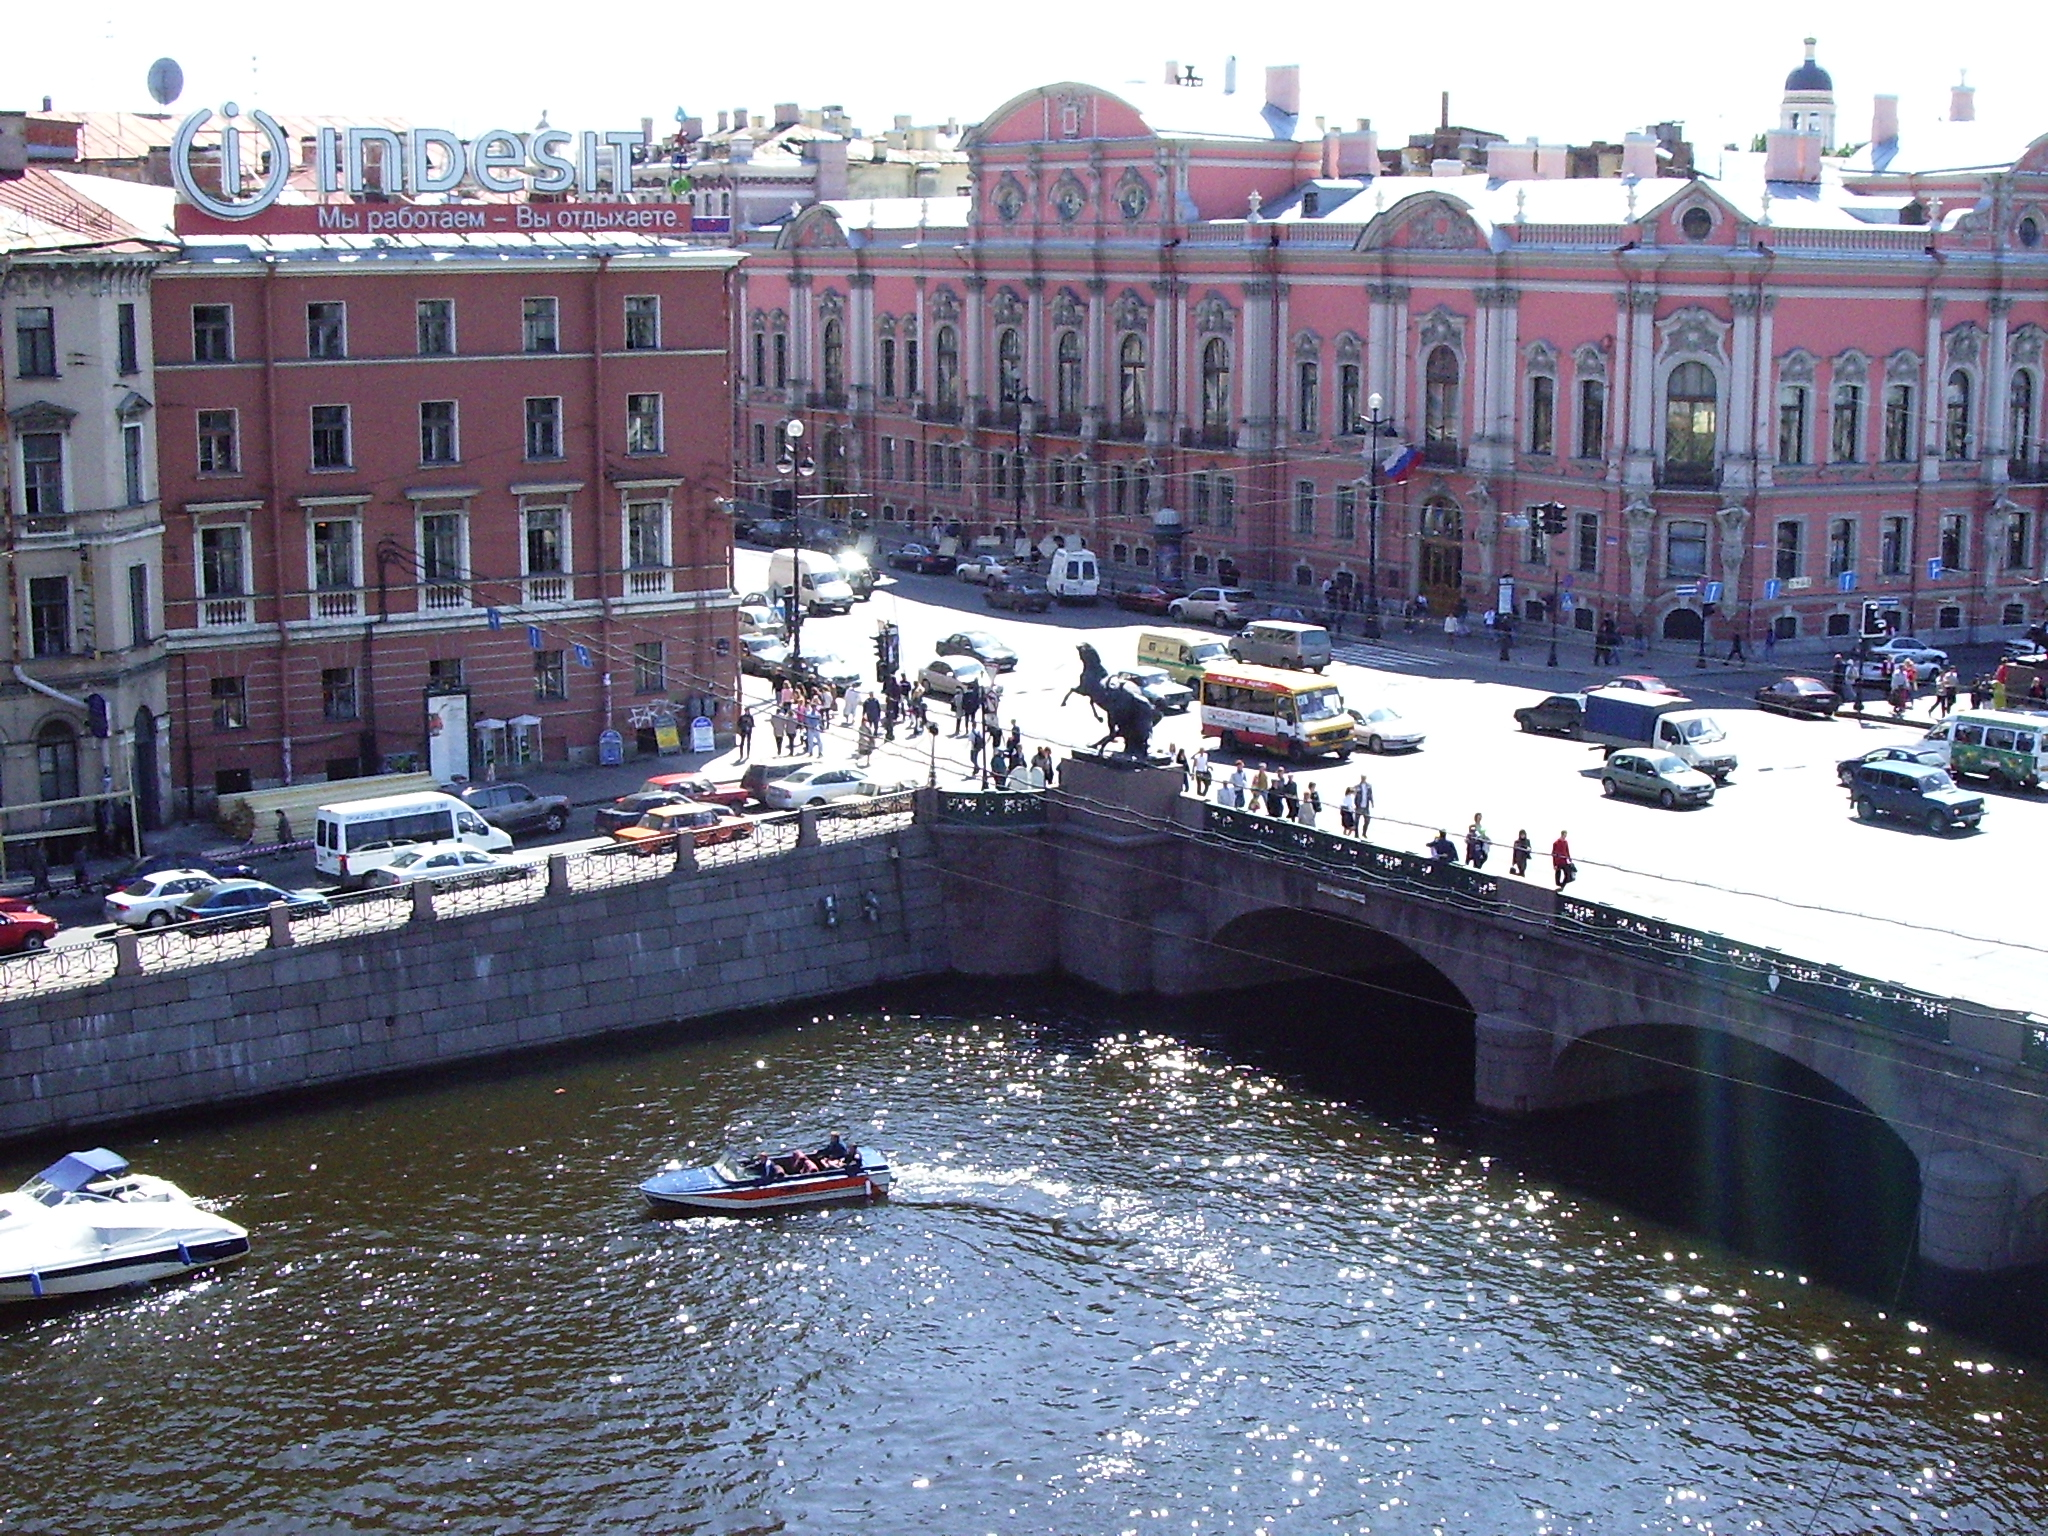
\includegraphics[width=10.8cm]{IMGP2770.PS}
%\caption{Caption goes here}
\end{figure}
%\clearpage

\vspace{-7cm}
}
{\red\fontsize{10pt}{18pt}\selectfont
\qquad P.A.Bolokhov, S.G.Nibbelink, M.Pospelov, hep-ph/0505029

\qquad We thank L.Smolin, N.Arkani-Hamed, M.Voloshin and M.Shifman

\qquad --- University of Guelph

\qquad --- University of Victoria

\qquad --- Perimeter Institute

}

\end{slide}
}

%%%%%%%%%%%%%%%%%%%%%%%%%%%%%%  SLIDE %%%%%%%%%%%%%%%%%%%%%%%%%%%%%%%%%%%%%%%
%%
%%\overlays{10}
%%{
%%\begin{slide}[Blinds]{ Title }
%%
%%
%%\end{slide}
%%}
%%
%%%%%%%%%%%%%%%%%%%%%%%%%%%%%%  SLIDE %%%%%%%%%%%%%%%%%%%%%%%%%%%%%%%%%%%%%%%

\end{document}
